\section{Course Management}
Another important sector in which AllSpark is involved is provide formation
courses and certifications for IT professionals. The teacher personal for
these courses are selected and trained among the developers and sysadmins
who works for AllSpark. 

The importance of this sector is underlined by the growing need for this
kind of certifications in many fields of information technologies related
applications.

The aim of AllSpark is to provide a service to many professionals who need
to certificate their knowledge and experience in various fields. On the
other hand this is a possibility to gain renown as a reliable authority for
delivering these services.

Organizing this section particular attention has been posed in defining
compatible timetables among the different courses, and assure the
up-to-date state of the study material and case studies presented.

The selection of the lecturers is also a vital task in order to organize a
successful course. AllSpark gives major importance to the experience of
their workers and to their ability in giving lectures, when selects the
lecturer for a course.

\subsection{Timetable management}
This process, represented in figure \ref{2img:timetable}  describes the
procedure needed in order to provide a consistent and non overlapping
schedule of the course.

Is important to provide an allocation that respect the possible
dependencies among different courses and avoids overlapping among lectures
of different courses.

\begin{figure}[!ht]
\centering
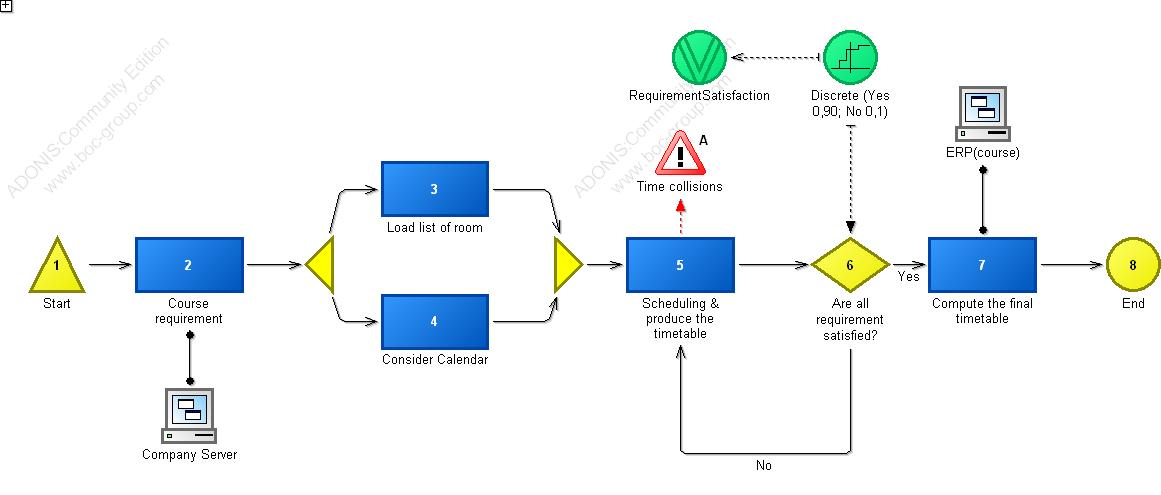
\includegraphics[scale=0.50,angle=90]{assign2/adonis/imgs/timetable.jpg}
\caption{Definition of the courses timetable}
\label{2img:timetable}
\end{figure}

\subsubsection{Path Analysis}
The results of the path analysis show that the most probable path
correspond to a situation where there are no problems in the flow.

\begin{table}[ht!]
\centering
\begin{tabular}{|l|l|l|l|l|}
\hline
Path&Probability&Execution time&Cycle time&Costs\\
\hline
1&0,898000&00:000:00:47:00&00:000:00:46:00&9,000000\\
\hline
2&0,093000&00:000:00:57:00&00:000:00:56:00&9,500000\\
\hline
3&0,008000&00:000:01:07:00&00:000:01:06:00&10,000000\\
\hline
4&0,001000&00:000:01:17:00&00:000:01:16:00&10,500000\\
\hline
\end{tabular}
\end{table}

\begin{alltt}
Probability:   89,8000%
Execution time:  00:000:00:47:00
Waiting time:  00:000:00:00:00
Resting time:  00:000:00:00:00
Transport time:  00:000:00:00:00
Cycle time:  00:000:00:46:00
Costs:  9,000000

Timetable 0.1 (Business process model)
========================================
Process start: Start
Activity: Course requirement
Parallelity: Parallelity-33508
    *
    Activity: Load list of room
    *
    Activity: Consider Calendar
Merging: Merging-33536
Activity: Scheduling & produce the timetable
Decision: Are all requirement satisfied? --> RequirementSatisfaction='Yes'
Activity: Compute the final timetable
End: End
\end{alltt}

\subsubsection{Capacity Analysis}
The table \ref{2tab:timetab} shows the results of capacity analysis.
There are no activities which are iterated more times than the others,
even due to the simplicity of this process.

\begin{landscape}
\centering
\begin{table}
{\tiny
\begin{tabular}{|l|l|l|l|l|l|l|}
Business process&Activity&Performer&Number&Execution time&Cycle
time&Costs\\
\hline
Timetable 0.1&&&&00:000:00:48:01&00:000:00:47:01&9,051000\\
\hline
&Compute the final timetable &&1,000000&00:000:00:02:00&&0,100000\\
\hline
&&Secretary &1,000000&00:000:00:02:00&&0,100000\\
\hline
&Scheduling \& produce the timetable &&1,102000&00:000:00:11:01&&0,551000\\
\hline
&&Secretary &1,102000&00:000:00:11:01&&0,551000\\
\hline
&Load list of room &&1,000000&00:000:00:01:00&&0,100000\\
\hline
&&Secretary &1,000000&00:000:00:01:00&&0,100000\\
\hline
&Consider Calendar &&1,000000&00:000:00:04:00&&0,300000\\
\hline
&&Secretary &1,000000&00:000:00:04:00&&0,300000\\
\hline
&Course requirement &&1,000000&00:000:00:30:00&&8,000000\\
\hline
&&Secretary &1,000000&00:000:00:30:00&&8,000000\\
\hline
Total&&&&00:000:00:48:01&&9,051000\\
\hline
\end{tabular}
}
\caption{Scheduling of timetable, capacity analysis} 
\label{2tab:timetab}
\end{table}
\end{landscape}





\subsection{Course organization}
This process is one of the most important in this area, in fact it manages
the effective organization of a course. During this process the attention
is focused, on a firs phase on the teacher selection and the gathering of
course material and planning definition.

If needed the people selected for the teacher role can be trained on the
course methodologies. After this first phase, are preformed  some
activities regarding the definition of the courses structure, the presence
of practical lessons, possible correlation with other courses and the
examination details.

All these informations are then integrated and published. The structure of
this process can be seen in figure \ref{2img:course_organization}.

\begin{figure}[!ht]
\centering
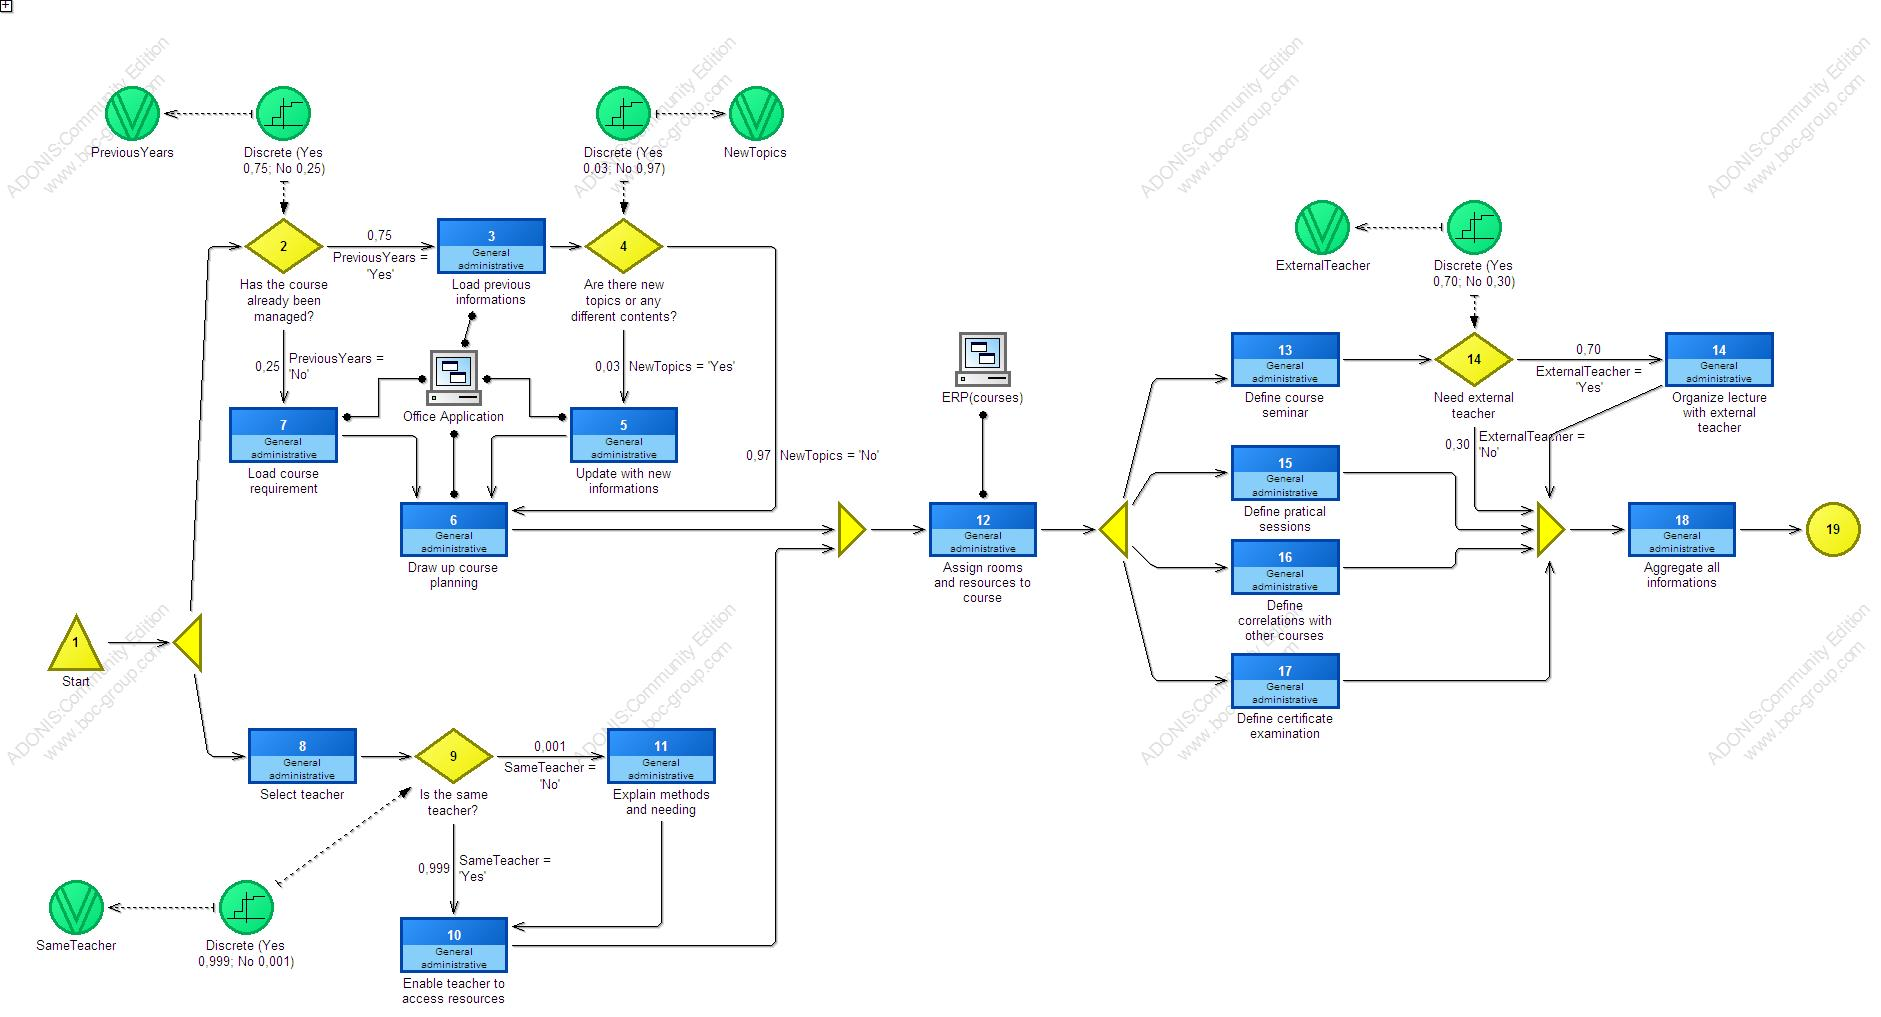
\includegraphics[scale=0.27, angle=90]{assign2/adonis/imgs/course_organization.jpg}
\caption{Organization of a formative course}
\label{2img:course_organization}
\end{figure}


\subsubsection{Path Analysis}
The difference in cost between the two most probable path is given by the
need of training new teachers or hiring external ones.

\begin{table}[ht!]
\centering
\begin{tabular}{|l|l|l|l|l|}
\hline
Path&Probability&Execution time&Cycle time&Costs\\
\hline
1&0,501000&00:000:05:15:00&00:000:03:41:00&418,500000\\
\hline
2&0,207000&00:000:03:15:00&00:000:01:41:00&168,500000\\
\hline
3&0,188000&00:000:05:15:00&00:000:03:41:00&418,600000\\
\hline
4&0,084000&00:000:03:15:00&00:000:01:41:00&168,600000\\
\hline
5&0,012000&00:000:06:15:00&00:000:04:34:00&438,500000\\
\hline
6&0,008000&00:000:04:15:00&00:000:02:34:00&188,500000\\
\hline
\end{tabular}
\end{table}

\begin{alltt}
Probability:   50,1000%
Execution time:  00:000:05:15:00
Waiting time:  00:000:00:00:00
Resting time:  00:000:00:00:00
Transport time:  00:000:00:00:00
Cycle time:  00:000:03:41:00
Costs:  418,500000

Course Organization 0.1 (Business process model)
========================================
Process start: Start
Parallelity: Parallelity-33578
    *
    Decision: Has the course already been managed? --> PreviousYears = 'Yes'
    Activity: Load previous informations
    Decision: Are there new topics or any different contents? --> NewTopics = 'No'
    Activity: Draw up course planning
    *
    Activity: Select teacher
    Decision: Is the same teacher? --> SameTeacher = 'Yes'
    Activity: Enable teacher to access resources
Merging: Merging-34785
Activity: Assign rooms and resources to course
Parallelity: Parallelity-34816
    *
    Activity: Define course seminar
    Decision: Need external teacher --> ExternalTeacher = 'Yes'
    Activity: Organize lecture with external teacher
    *
    Activity: Define pratical sessions
    *
    Activity: Define correlations with other courses
    *
    Activity: Define certificate examination
Merging: Merging-34835
Activity: Aggregate all informations
End: End-34847
\end{alltt}

\subsubsection{Capacity Analysis}
The table \ref{2tab:course_org} shows the results of capacity analysis.
As is possible to see from this table one of the most costly activity is
to organize lectures with external teachers. So AllSpark should avoid this
policy as possible.


\begin{landscape}
\centering
\begin{table}
{\tiny
\begin{tabular}{|l|l|l|l|l|l|l|}
Business process&Activity&Performer&Number&Execution time&Cycle
time&Costs\\
\hline
Course Organization 0.1&&&&00:000:04:40:44&00:000:03:06:35&344,737600\\
\hline
&Load previous informations &&0,724000&00:000:00:02:54&&0,217200\\
\hline
&&Secretary &0,724000&00:000:00:02:54&&0,217200\\
\hline
&Update with new informations &&0,023000&00:000:00:01:23&&0,460000\\
\hline
&&Secretary &0,023000&00:000:00:01:23&&0,460000\\
\hline
&Draw up course planning &&1,000000&00:000:00:40:00&&9,000000\\
\hline
&&Secretary &1,000000&00:000:00:40:00&&9,000000\\
\hline
&Load course requirement &&0,276000&00:000:00:01:06&&0,110400\\
\hline
&&Secretary &0,276000&00:000:00:01:06&&0,110400\\
\hline
&Enable teacher to access resources &&1,000000&00:000:00:01:00&&0,200000\\
\hline
&&Secretary &1,000000&00:000:00:01:00&&0,200000\\
\hline
&Assign rooms and resources to course &&1,000000&00:000:00:10:00&&1,000000\\
\hline
&&Secretary &1,000000&00:000:00:10:00&&1,000000\\
\hline
&Define course seminar &&1,000000&00:000:00:30:00&&30,000000\\
\hline
&&Secretary &1,000000&00:000:00:30:00&&30,000000\\
\hline
&Define pratical sessions &&1,000000&00:000:00:20:00&&3,000000\\
\hline
&&Secretary &1,000000&00:000:00:20:00&&3,000000\\
\hline
&Define correlations with other courses &&1,000000&00:000:00:10:00&&2,000000\\
\hline
&&Secretary &1,000000&00:000:00:10:00&&2,000000\\
\hline
&Define certificate examination &&1,000000&00:000:00:20:00&&2,000000\\
\hline
&&Secretary &1,000000&00:000:00:20:00&&2,000000\\
\hline
&Aggregate all informations &&1,000000&00:000:00:10:00&&1,000000\\
\hline
&&Secretary &1,000000&00:000:00:10:00&&1,000000\\
\hline
&Organize lecture with external teacher &&0,703000&00:000:01:24:22&&175,750000\\
\hline
&&Secretary &0,703000&00:000:01:24:22&&175,750000\\
\hline
&Select teacher &&1,000000&00:000:00:50:00&&120,000000\\
\hline
&&Secretary &1,000000&00:000:00:50:00&&120,000000\\
\hline
Total&&&&00:000:04:40:44&&344,737600\\
\hline
\end{tabular}
}
\caption{Capacity analysis for the process of organize a course} 
\label{2tab:course_org}
\end{table}
\end{landscape}




\subsection{Course Material Management}
This process, as in figure \ref{2img:course_material}, represents the way
in which AllSpark manages the material needed as support for a course.
Obviously in order to provide a right choice of material is necessary to
analyze deeply the course scope.

Other important things are the quality of the material offered and its
consistency, in terms of completeness and correctness. AllSpark uses its
own infrastructure in order to offer a sort of reliable repository of
course material and documentation. The access to this repository is
scheduled consistently with the course schedule.

\begin{figure}[!ht]
\centering
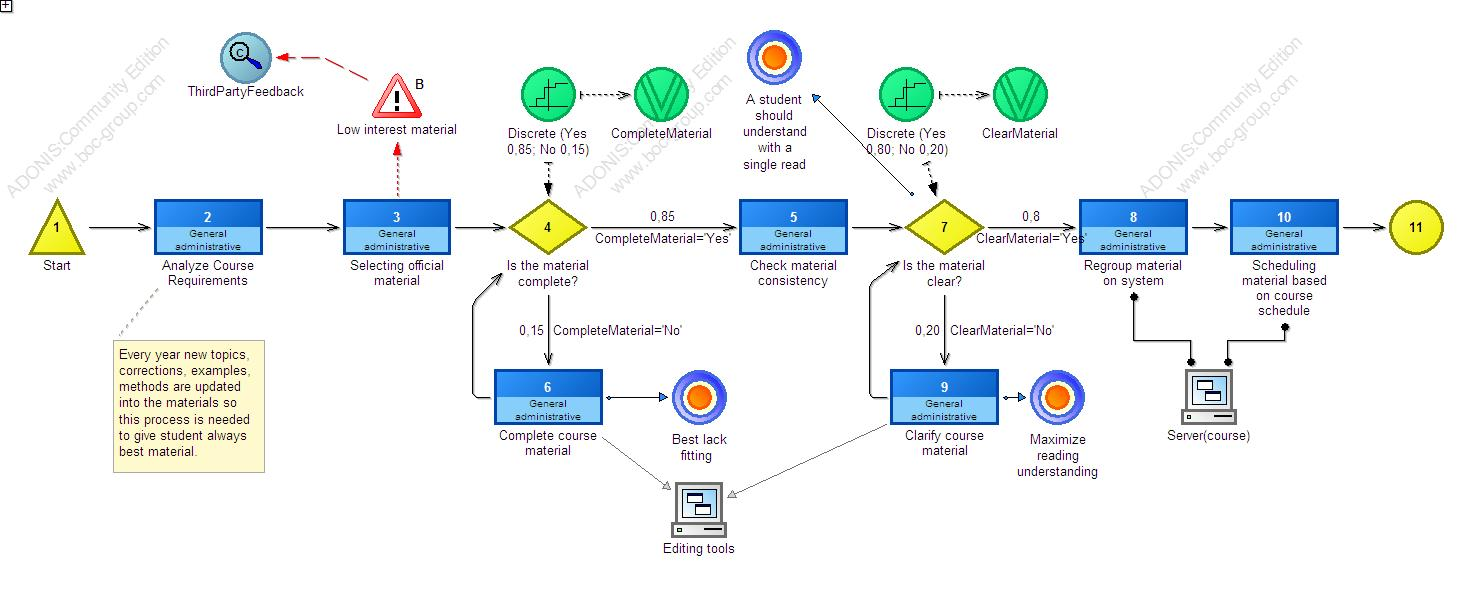
\includegraphics[scale=0.35, angle=90]{assign2/adonis/imgs/course_material.jpg}
\caption{Gathering and evaluation of course material}
\label{2img:course_material}
\end{figure}


\subsubsection{Path Analysis}
The most probable path is the case in which the material for the course is
up to date, this brings to a reduce of the costs in respect of the other
cases.

\begin{table}[ht!]
\centering
\begin{tabular}{|l|l|l|l|l|}
\hline
Path&Probability&Execution time&Cycle time&Costs\\
\hline
1&0,683000&00:000:02:20:00&00:000:02:20:00&51,500000\\
\hline
2&0,136000&00:000:02:40:00&00:000:02:40:00&60,500000\\
\hline
3&0,101000&00:000:02:40:00&00:000:02:40:00&61,500000\\
\hline
4&0,025000&00:000:03:00:00&00:000:03:00:00&70,500000\\
\hline
5&0,024000&00:000:03:00:00&00:000:03:00:00&69,500000\\
\hline
6&0,016000&00:000:03:00:00&00:000:03:00:00&71,500000\\
\hline
7&0,005000&00:000:03:20:00&00:000:03:20:00&78,500000\\
\hline
8&0,004000&00:000:03:20:00&00:000:03:20:00&80,500000\\
\hline
9&0,003000&00:000:03:20:00&00:000:03:20:00&81,500000\\
\hline
10&0,001000&00:000:04:20:00&00:000:04:20:00&107,500000\\
\hline
11&0,001000&00:000:03:20:00&00:000:03:20:00&79,500000\\
\hline
12&0,001000&00:000:04:00:00&00:000:04:00:00&96,500000\\
\hline
\end{tabular}
\end{table}

\begin{alltt}
Probability:   68,3000%
Execution time:  00:000:02:20:00
Waiting time:  00:000:00:00:00
Resting time:  00:000:00:00:00
Transport time:  00:000:00:00:00
Cycle time:  00:000:02:20:00
Costs:  51,500000

Course material 0.1 (Business process model)
========================================
Process start: Start
Activity: Analyze Course Requirements
Activity: Selecting official material
Decision: Is the material complete? --> CompleteMaterial='Yes'

Activity: Check material consistency
Decision: Is the material clear? --> ClearMaterial='Yes'
Activity: Regroup material on system
Activity: Scheduling material based on course schedule
End: End-35061
\end{alltt}

\subsubsection{Capacity Analysis}
The table \ref{2tab:material} shows the results of capacity analysis.
This analysis shows hot the cost rises for activities which need a active
human work for long time, as analyzing the consistency of the material.

\begin{landscape}
\centering
\begin{table}
{\tiny
\begin{tabular}{|l|l|l|l|l|l|l|}
Business process&Activity&Performer&Number&Execution time&Cycle
time&Costs\\
\hline
Course material 0.1&&&&00:000:02:28:35&00:000:02:28:35&55,547000\\
\hline
&Analyze Course Requirements &&1,000000&00:000:00:15:00&&1,000000\\
\hline
&&Secretary &1,000000&00:000:00:15:00&&1,000000\\
\hline
&Selecting official material &&1,000000&00:000:01:00:00&&20,000000\\
\hline
&&Secretary &1,000000&00:000:01:00:00&&20,000000\\
\hline
&Check material consistency &&1,000000&00:000:01:00:00&&30,000000\\
\hline
&&Secretary &1,000000&00:000:01:00:00&&30,000000\\
\hline
&Scheduling material based on course schedule &&1,000000&00:000:00:02:00&&0,200000\\
\hline
&&Secretary &1,000000&00:000:00:02:00&&0,200000\\
\hline
&Regroup material on system &&1,000000&00:000:00:03:00&&0,300000\\
\hline
&&Secretary &1,000000&00:000:00:03:00&&0,300000\\
\hline
&Complete course material &&0,186000&00:000:00:03:43&&1,860000\\
\hline
&&Secretary &0,186000&00:000:00:03:43&&1,860000\\
\hline
&Clarify course material &&0,243000&00:000:00:04:52&&2,187000\\
\hline
&&Secretary &0,243000&00:000:00:04:52&&2,187000\\
\hline
Total&&&&00:000:02:28:35&&55,547000\\
\hline
\end{tabular}
}
\caption{Capacity analysis for the process of organizing course material} 
\label{2tab:material}
\end{table}
\end{landscape}




\subsection{Examinations}
At the end of the most of the courses, an official examination is planned,
this is very important in order to achieve the goal of gain renown as a
certification authority. In fact the AllSpark standard in this area is to
keep the level of the course and of the examination quite high, in order to
add an ulterior value to our certifications.

Often AllSpark provides examination service for other Authorities, in this
case is necessary to retrieve from them the original text and organize the
examination over that particular test.

Difficulties on this process can be originated by the ambiguos nature of
some examination modalities, like for example open questions, which can
lead to misjudgement and wrong results in the evaluation.
The process is described by figure \ref{2img:examination}.

\begin{figure}[!ht]
\centering
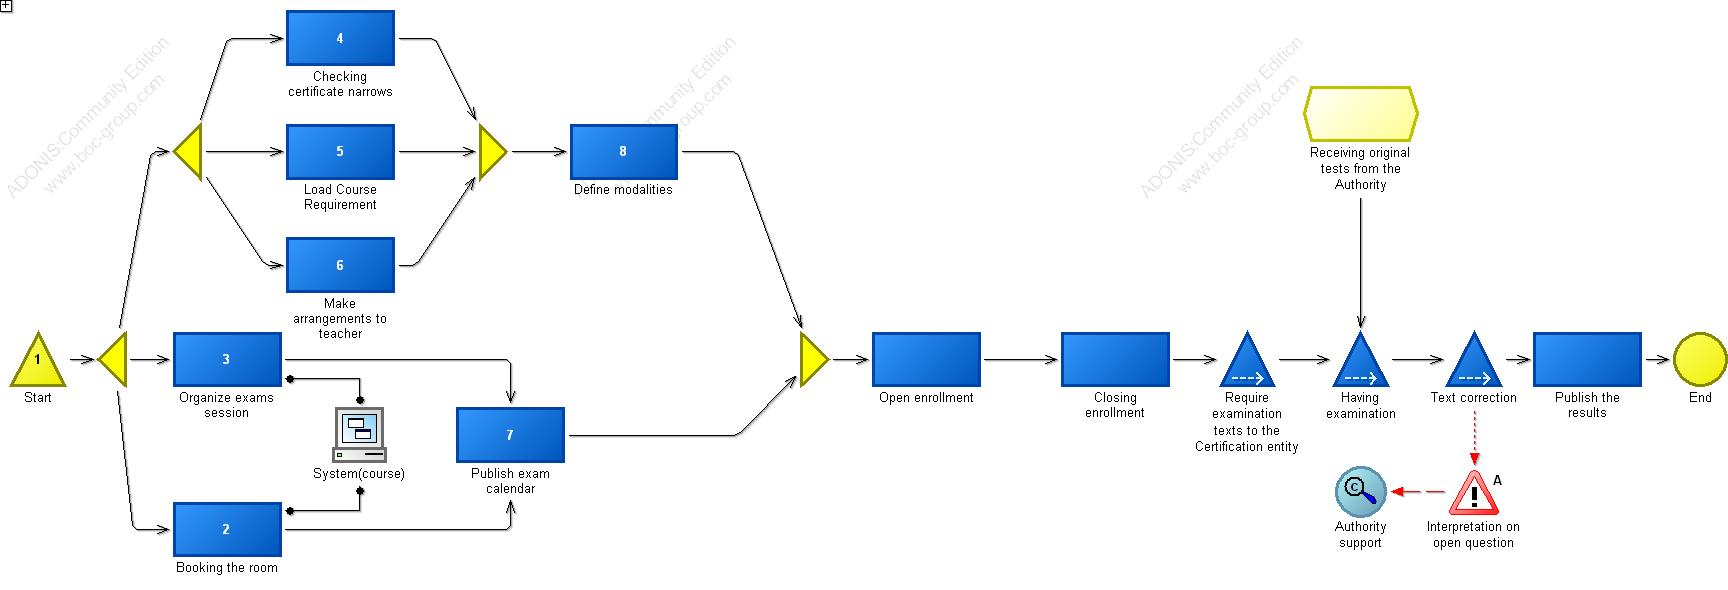
\includegraphics[scale=0.35, angle=90]{assign2/adonis/imgs/examination.jpg}
\caption{Organization of an examination test}
\label{2img:examination}
\end{figure}



\subsubsection{Path Analysis}
This analysis shows only one possible path, in fact the process is a set
of activities with no condition.

\begin{table}[ht!]
\centering
\begin{tabular}{|l|l|l|l|l|}
\hline
1&1,000000&00:001:01:57:00&00:001:01:31:00&94,100000\\
\hline
\end{tabular}
\end{table}

\begin{alltt}
Probability:   100,0000%
Execution time:  00:001:01:57:00
Waiting time:  00:000:00:00:00
Resting time:  00:000:00:00:00
Transport time:  00:000:00:00:00
Cycle time:  00:001:01:31:00
Costs:  94,100000

Examination 0.1 (Business process model)
========================================
Process start: Start
Parallelity: Parallelity-35109
    *
    Activity: Booking the room
    Activity: Publish exam calendar
    *
    Activity: Organize exams session
    Activity: Publish exam calendar
    *
    Parallelity: Parallelity-35154
        *
        Activity: Load Course Requirement
        *
        Activity: Checking certificate narrows
        *
        Activity: Make arrangements to teacher
    Merging: Merging-35157
    Activity: Define modalities
Merging: Merging-35174
Activity: Open enrollment
Activity: Closing enrollment
Activity: Require original test
Activity: Test correction
Activity: Publish the results
End: End
\end{alltt}

\subsubsection{Capacity Analysis}
The table \ref{2tab:exam} shows the results of capacity analysis.
The analysis shows that the most costly activity is the coorrection of the
tests, but is considered better than an automatic corrector.

\begin{landscape}
\centering
\begin{table}
{\tiny
\begin{tabular}{|l|l|l|l|l|l|l|}
Business process&Activity&Performer&Number&Execution time&Cycle
time&Costs\\
\hline
Examination 0.1&&&&00:001:01:57:00&00:001:01:31:00&94,100000\\
\hline
&Load Course Requirement &&1,000000&00:000:00:02:00&&0,200000\\
\hline
&&Secretary &1,000000&00:000:00:02:00&&0,200000\\
\hline
&Checking certificate narrows &&1,000000&00:000:00:10:00&&1,000000\\
\hline
&&Secretary &1,000000&00:000:00:10:00&&1,000000\\
\hline
&Booking the room &&1,000000&00:000:00:02:00&&0,100000\\
\hline
&&Secretary &1,000000&00:000:00:02:00&&0,100000\\
\hline
&Open enrollment &&1,000000&00:000:00:02:00&&0,700000\\
\hline
&&Secretary &1,000000&00:000:00:02:00&&0,700000\\
\hline
&Organize exams session &&1,000000&00:000:00:10:00&&0,800000\\
\hline
&&Secretary &1,000000&00:000:00:10:00&&0,800000\\
\hline
&Define modalities &&1,000000&00:000:00:30:00&&3,000000\\
\hline
&&Secretary &1,000000&00:000:00:30:00&&3,000000\\
\hline
&Make arrangements to teacher &&1,000000&00:000:00:10:00&&2,000000\\
\hline
&&Secretary &1,000000&00:000:00:10:00&&2,000000\\
\hline
&Publish exam calendar &&2,000000&00:000:00:02:00&&0,800000\\
\hline
&&Secretary &2,000000&00:000:00:02:00&&0,800000\\
\hline
&Closing enrollment &&1,000000&00:000:00:02:00&&0,300000\\
\hline
&&Secretary &1,000000&00:000:00:02:00&&0,300000\\
\hline
&Publish the results &&1,000000&00:000:00:02:00&&0,200000\\
\hline
&&Secretary &1,000000&00:000:00:02:00&&0,200000\\
\hline
&Require original test &&1,000000&00:000:00:45:00&&5,000000\\
\hline
&&Secretary &1,000000&00:000:00:45:00&&5,000000\\
\hline
&Test correction &&1,000000&00:001:00:00:00&&80,000000\\
\hline
&&Secretary &1,000000&00:001:00:00:00&&80,000000\\
\hline
Total&&&&00:001:01:57:00&&94,100000\\
\hline
\end{tabular}
}
\caption{Capacity analysis for the process of organize examination} 
\label{2tab:exam}
\end{table}
\end{landscape}




\subsection{Certification management}
This process permits to manage the delivery of the certification to the
candidates who passed the examination. Often the certification is provided
by an external organization, for which AllSpark acts as an examination
authority. In this case in necessary to send them the list of approved
candidates, and retrieve the certification documents.

This process can handle the case in which a single certification is
considered as a hierarchy of other certifications, in this case all the
other documents are equally retrieved.

The image in figure \ref{2img:certification} describes this process. Here
the final document is customized with AllSpark logo and information.

\begin{figure}[!ht]
\centering
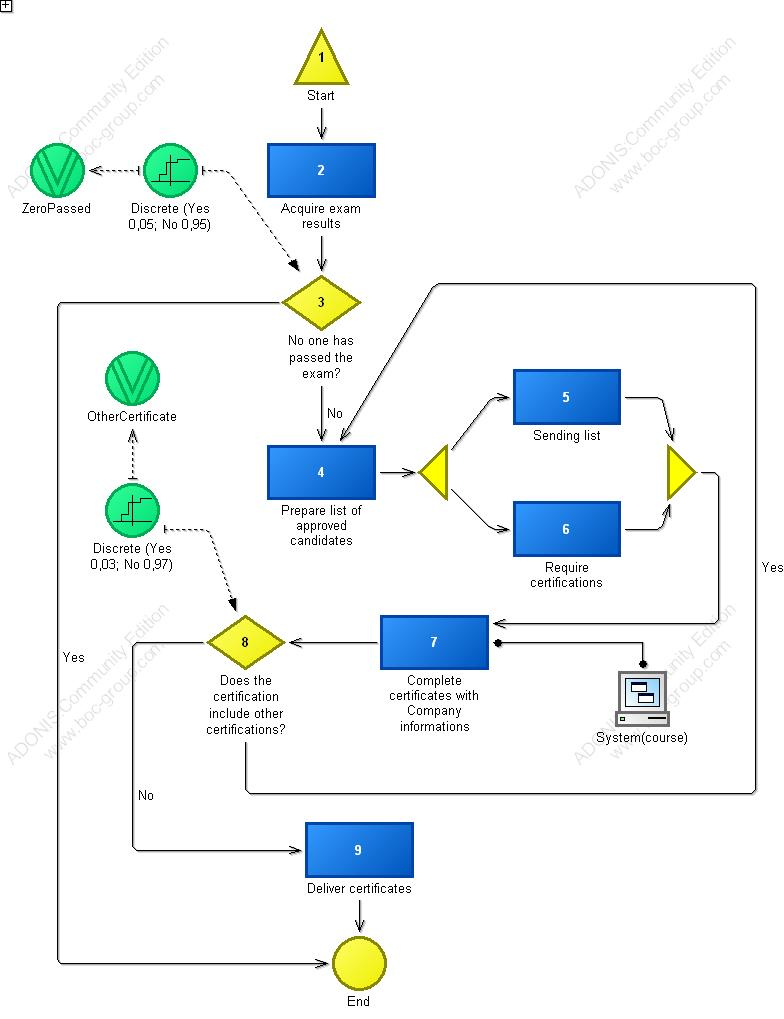
\includegraphics[scale=0.55]{assign2/adonis/imgs/certification.jpg}
\caption{Delivery of certification documents}
\label{2img:certification}
\end{figure}




\subsubsection{Path Analysis}
The most probable path corresponds to an exam which delivers only one
certification and some students have passed.

\begin{table}[ht!]
\centering
\begin{tabular}{|l|l|l|l|l|}
\hline
Path&Probability&Execution time&Cycle time&Costs\\
\hline
Path&Probability&Execution time&Cycle time&Costs\\
\hline
1&0,921000&00:000:00:54:00&00:000:00:49:00&13,700000\\
\hline
2&0,044000&00:000:00:02:00&00:000:00:02:00&0,100000\\
\hline
3&0,034000&00:000:01:41:00&00:000:01:31:00&26,400000\\
\hline
4&0,001000&00:000:02:28:00&00:000:02:13:00&39,100000\\
\hline
\end{tabular}
\end{table}

\begin{alltt}
Probability:   92,1000%
Execution time:  00:000:00:54:00
Waiting time:  00:000:00:00:00
Resting time:  00:000:00:00:00
Transport time:  00:000:00:00:00
Cycle time:  00:000:00:49:00
Costs:  13,700000

Certification 0.1 (Business process model)
========================================
Process start: Start
Activity: Acquire exam results
Decision: No one has passed the exam? --> ZeroPassed='No'
Activity: Prepare list of approved candidates
Parallelity: Parallelity-35259
    *
    Activity: Sending list
    *
    Activity: Require certifications
Merging: Merging-35265
Activity: Complete certificates with Company informations
Decision: Does the certification include other certifications? --> OtherCertificate='No'

Activity: Deliver certificates
End: End
\end{alltt}

\subsubsection{Capacity Analysis}
The table \ref{2tab:exam} shows the results of capacity analysis.
There are no particular feature in this analysis, considering that all the
activities are executed a fair number of times and with similar costs.

\begin{landscape}
\centering
\begin{table}
{\tiny
\begin{tabular}{|l|l|l|l|l|l|l|}
Business process&Activity&Performer&Number&Execution time&Cycle
time&Costs\\
\hline
Certification 0.1&&&&00:000:00:53:12&00:000:00:48:16&13,506200\\
\hline
&Acquire exam results &&1,000000&00:000:00:02:00&&0,100000\\
\hline
&&Secretary &1,000000&00:000:00:02:00&&0,100000\\
\hline
&Prepare list of approved candidates &&0,988000&00:000:00:01:59&&0,197600\\
\hline
&&Secretary &0,988000&00:000:00:01:59&&0,197600\\
\hline
&Sending list &&0,988000&00:000:00:04:56&&0,494000\\
\hline
&&Secretary &0,988000&00:000:00:04:56&&0,494000\\
\hline
&Require certifications &&0,988000&00:000:00:29:38&&2,964000\\
\hline
&&Secretary &0,988000&00:000:00:29:38&&2,964000\\
\hline
&Complete certificates with Company informations &&0,988000&00:000:00:09:53&&8,892000\\
\hline
&&Secretary &0,988000&00:000:00:09:53&&8,892000\\
\hline
&Deliver certificates &&0,954000&00:000:00:04:46&&0,858600\\
\hline
&&Secretary &0,954000&00:000:00:04:46&&0,858600\\
\hline
Total&&&&00:000:00:53:12&&13,506200\\
\hline
\end{tabular}
}
\caption{Capacity analysis for the process of delivering the certifications} 
\label{2tab:certs}
\end{table}
\end{landscape}

